\documentclass[tikz,border=5pt]{standalone}
\usepackage[utf8]{inputenc}
\usepackage[T1]{fontenc}
\usepackage{amsmath,amssymb}
\usepackage{lmodern}
\usetikzlibrary{arrows.meta}

\definecolor{ink}{HTML}{1d1d1f}
\definecolor{sub}{HTML}{515154}
\definecolor{muted}{HTML}{6e6e73}
\definecolor{green}{HTML}{1a7f37}
\definecolor{greenbright}{HTML}{30d158}
\definecolor{greenfill}{HTML}{dcf7e3}
\definecolor{red}{HTML}{d70015}
\definecolor{redbright}{HTML}{ff453a}
\definecolor{redfill}{HTML}{ffe5e3}

\begin{document}
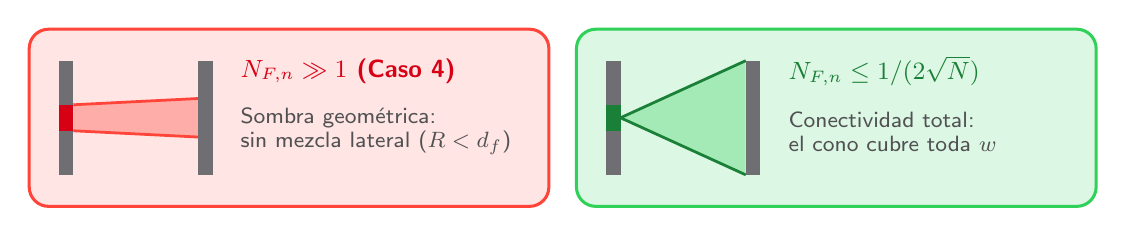
\begin{tikzpicture}[font=\sffamily,>=Stealth]

% ===================== CAJA IZQUIERDA: SOMBRA GEOMÉTRICA =====================
\draw[redbright,fill=redfill,rounded corners=7pt,line width=1.1pt] (0,0) rectangle (6.60,2.25);

% Placas y haz estrecho
\fill[muted] (0.38,0.40) rectangle (0.56,1.85);
\fill[red]   (0.38,0.96) rectangle (0.56,1.29);
\fill[redbright,opacity=0.35] (0.56,0.96) -- (2.15,0.88) -- (2.15,1.37) -- (0.56,1.29) -- cycle;
\draw[redbright,line width=1.0pt] (0.56,0.96) -- (2.15,0.88);
\draw[redbright,line width=1.0pt] (0.56,1.29) -- (2.15,1.37);
\fill[muted] (2.15,0.40) rectangle (2.33,1.85);

\node[anchor=west,font=\sffamily\small\bfseries,text=red] at (2.56,1.72)
  {$N_{F,n} \gg 1$ (Caso 4)};
\node[anchor=west,font=\sffamily\footnotesize,text=sub,align=left] at (2.56,0.95)
  {Sombra geométrica:\\[-1pt]sin mezcla lateral ($R < d_f$)};

% ===================== CAJA DERECHA: CONECTIVIDAD TOTAL =====================
\draw[greenbright,fill=greenfill,rounded corners=7pt,line width=1.1pt] (6.95,0) rectangle (13.55,2.25);

% Placas y cono completo
\fill[muted] (7.33,0.40) rectangle (7.51,1.85);
\fill[green] (7.33,0.96) rectangle (7.51,1.29);
\fill[greenbright,opacity=0.32] (7.51,1.125) -- (9.10,0.40) -- (9.10,1.85) -- cycle;
\draw[green,line width=1.0pt] (7.51,1.125) -- (9.10,0.40);
\draw[green,line width=1.0pt] (7.51,1.125) -- (9.10,1.85);
\fill[muted] (9.10,0.40) rectangle (9.28,1.85);

\node[anchor=west,font=\sffamily\small\bfseries,text=green] at (9.52,1.72)
  {$N_{F,n} \le 1/(2\sqrt{N})$};
\node[anchor=west,font=\sffamily\footnotesize,text=sub,align=left] at (9.52,0.95)
  {Conectividad total:\\[-1pt]el cono cubre toda $w$};

\end{tikzpicture}
\end{document}
